\subsection{Larvitrampas}
\label{sec:densidad-vectorial-larvitrampas}
Las larvitrampas son, dispositivos artificiales creados con el fin de simular el habitad del
vector de forma controlada. El diseño más simple (\figref{fig:cap3-larvitrampas}) es una sección
radial de una llanta llena de agua \cite{world2009dengue}.

\begin{figure}
\centering
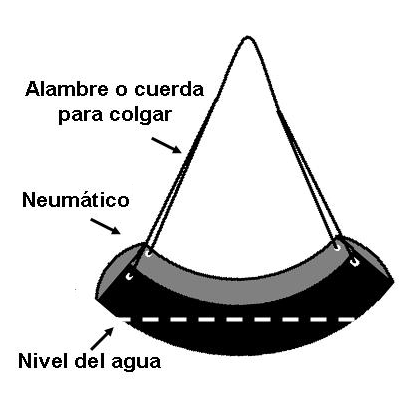
\includegraphics[width=0.4\textwidth]{capitulo-3/graphics/larvitrampa.png}
\caption{\label{fig:cap3-larvitrampas} Diseño de una larvitrampa(Tomado de
\cite{manualControlArg2009}).}
\end{figure}

Se basan en la detección del vector en su etapa larval
\cite{manualControlArg2009, MARQUES1993}, que brinda información sobre los patrones de actividad
espacial y estacional de ovipostura, y además, permiten reconocer las condiciones climáticas
favorables para la eclosión y desarrollo larvario \cite{manualControlArg2009}.

En las áreas infestadas, o con alto riesgo de infección con Aedes aegypti, la inspección debe
realizarse de forma periódica, según \cite{manualControlArg2009}, con el fin de :

\begin{itemize}
    \item Conocer la distribución del vector y el grado de infestación para establecer el nivel de riesgo de transmisión de dengue en las áreas geográficas infestadas.
    \item Detectar oportunamente la infestación en las áreas no infestadas.
    \item Detectar la introducción de Aedes aegypti en áreas no infestadas.
    \item Evaluación de acciones realizadas.
\end{itemize}

Las llantas o neumáticos son considerados como criaderos de alto riesgo
\cite{bisset2008distribucion, manrique1998desarrollo, ulloa1996abundancia}, donde, la
supervivencia y la duración del ciclo de vida en neumáticos son menores a los reportados para
otros tipos de contenedores \cite{manrique1998desarrollo}. Esto resalta la importancia de los
neumáticos como criaderos y blanco para el control del vector del dengue \cite{manrique1998desarrollo, ulloa1996abundancia}.

Las larvitrampas, construidas de neumáticos, permiten transformar estos criaderos de alto
riesgo en una herramienta para el control del vector del dengue mediante el reciclaje.

\subsection{Ovitrampa}
\label{sec:densidad-vectorial-ovitrampa}
Las ovitrampas constituyen un método sensible y económico para el monitoreo del Aedes aegypti y
útiles para determinar el comportamiento poblacional del vector y conocer las áreas de riesgo
entomológico\cite{cenaprece2013}. Su diseño estándar se encuentra compuesto por una jarra de
vidrio pintada de negro \cite{dengueUruguayCap1, world2009dengue}, equipada con una chapa de
madera o paleta de madera \cite{dengueUruguayCap1, world2009dengue, website:TimothyOvitrap2014,
manualControlArg2009}. Así mismo pueden utilizarse recipientes de plástico
\cite{website:TimothyOvitrap2014, cenaprece2013, manualControlArg2009, MARQUES1993} en reemplazo
de las jarras de vidrio por su bajo costo.


\begin{figure}
\centering
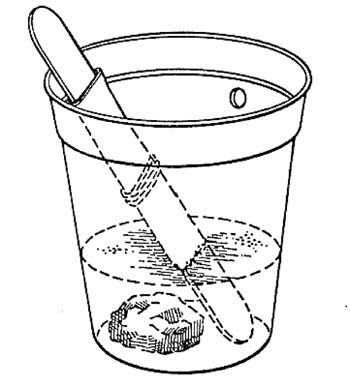
\includegraphics[width=0.3\textwidth]{capitulo-3/graphics/ovitrampa.jpg}
\caption{\label{fig:cap3-larvitrampas} Diseño de una ovitrampa (Tomado de
\cite{website:TimothyOvitrap2014}).}
\end{figure}

Las ovitrampas constituyen un método sensible y económico para el monitoreo del Aedes aegypti
\cite{cenaprece2013, world2009dengue}, y son útiles para determinar el comportamiento poblacional
del vector y conocer las áreas de riesgo entomológico \cite{cenaprece2013}. La información
proporcionada permite para determinar la distribución espacial y temporal de Aedes aegypti y otros
mosquitos \cite{dengueUruguayCap1, NINO2011}. Se pueden instalar y preparar en forma relativamente
rápida en grandes áreas \cite{world2009dengue}.


